\documentclass{techbrief}

\title{Tech Brief}
\title{Activities}
\date{January 2025}
\event{Special Report}

\usepackage{lipsum}

\begin{document}
\newgeometry{margin=1cm,headheight=3cm,includehead,includefoot}
\pagestyle{main}
\thispagestyle{title}
\pagenumbering{gobble}
\noindent

\lettrine[lines=2]{X}{imera} had a remarkable presence at the \textit{Joint
    Mathematics Meetings 2025}, drawing considerable interest from attendees.
Strategically located in the exhibit hall, our booth became a key attraction.
During the conference, we demonstrated Ximera's features and discussed our
upcoming initiatives. Five dedicated members of the Ximera team were present:
Jim Fowler, Tae Eun Kim, Jeff Kuan, Bart Snapp, and Paul Zachlin.

\begin{xframe}
    {\textbf{The Ximera booth}} operated during the following hours: Wednesday
    6:00pm--8:00pm, Thursday 9am--5pm, Friday 9am--5pm, and Saturday 9am--noon.
    Positioned in a corner just behind our proprietary competitors, our booth
    captured attention
    with a dynamic slideshow on a 100-inch screen.
    \begin{center}
        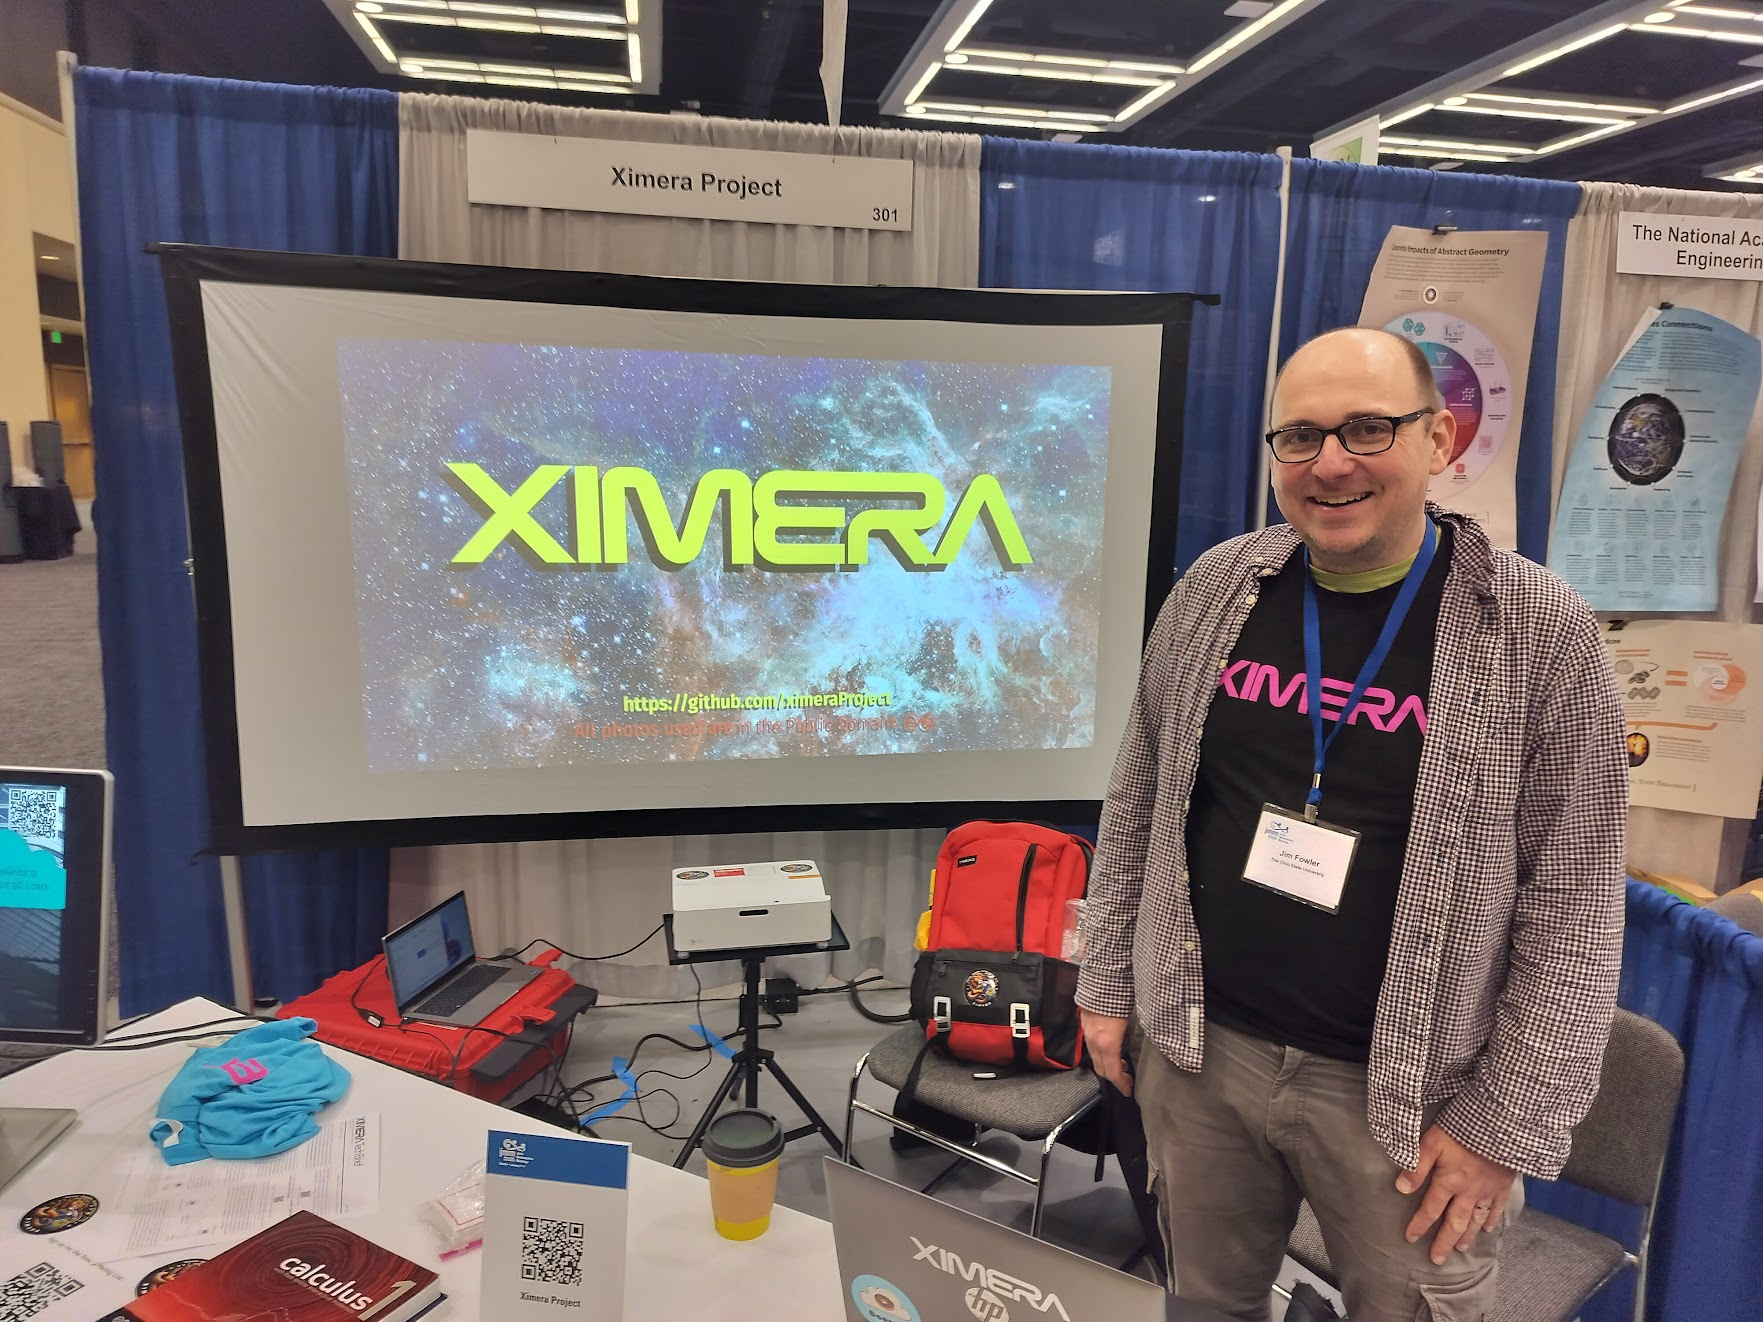
\includegraphics[width=.9\textwidth]{booth.jpg}
    \end{center}
    A computer monitor on the table displayed a video showcasing Ximera in
    action. We also featured bound demonstration copies of our calculus texts
    and
    \textit{Linear Algebra: An Interactive Approach} by Anna Davis and Paul
    Zachlin. 
\end{xframe}

\begin{xframe}
    {\bf New connections} were formed! We distributed approximately 60
    Ximera T-shirts, 70 User Manuals, 50 TechBriefs, and added 54 emails to our
    mailing list. Several attendees expressed interest in converting their
    existing
    \LaTeX\ content into Ximera, paving the way for potential collaborations.
    \begin{center}

        
\includegraphics[width=.15\textwidth]{../../missionPatch/missionPatch.png}\qquad\includegraphics[width=.3\textwidth]{../../criticalMathItem/criticalItem.pdf}
    \end{center}
    If you'd like Ximera T-shirts (more are on the way!) or stickers, please
    let us know, and we will
    fulfill your order with care. 
\end{xframe}

\break

\begin{xframe}
    \textbf{Presentations featuring Ximera}
    On Saturday, Paul Zachlin delivered a talk titled \textit{Enhancing our
        Linear
        Algebra OER with Additional Features}.

    The presentation introduced the book (co-authored with Anna Davis)
    \begin{center}
    \texttt{https://go.osu.edu/ila}
    \end{center}
    and highlighted new additions such as
    an Octave Tutorial and Review Exercises. Future plans for online resources,
    including those for a differential equations course, were also discussed.
    Approximately 20 participants attended this session.
\end{xframe}

\vfil

\begin{xframe}
    \textbf{Get started in Ximera} by checking out \textit{Ximera First Steps}
   \begin{center}\small
        \texttt{https://go.osu.edu/xfs}
    \end{center}
and please consider applying for the \textbf{Ximera Workshop 10}, in Columbus, Ohio May 12--14 here:
\begin{center}\small
    \texttt{https://ximera.org/workshops}
\end{center} 
\end{xframe}

\vfil
\begin{xframe}
    {\bfseries Intersections: Online Learning + Innovation in Higher
        Education} is a conference sponsored by the University of Florida. There will be several presentations featuring Ximera. See:
        \begin{center}\small
            \texttt{https://pwd.aa.ufl.edu/intersections/}
        \end{center}       
\end{xframe}



\begin{xframe}
    \textbf{Funding for the Ximera Project} is provided by
    a U.S.\ Department of Education Open Textbooks Pilot Program grant in the
    amount of \$2,125,000, from 2024--2026, with no external funding. In the
    past, the Ximera Project has
    also received support from NSF Grant DUE-1245433, the Shuttleworth
    Foundation, the Ohio State University
    Department of Mathematics, and the Affordable Learning Exchange at OSU.
\end{xframe}

\vfill

\end{document}